\section{Interfaces de usuarios}


A continuación se muestran las interfaces desarrolladas en PyQt5. Se busca mantener una estructura intuitiva y modular que facilite la configuración, ejecución y visualización del CA.

\begin{itemize}
	\item \textbf{Interfaz principal}
	
	La interfaz principal se divide en tres secciones: el espacio de evolución, ubicado en la parte superior izquierda, donde se visualiza la cuadrícula en la que evoluciona el autómata celular; el área de controles, situada en la parte inferior izquierda, que permite manipular la simulación (iniciar, pausar, reiniciar, avanzar o retroceder); y la sección de configuración, ubicada a la derecha, donde se especifican parámetros como la vecindad, las condiciones de frontera, los estados, los colores asociados y la regla de transición (Figura \ref{fig:ui_main}).
	
	\begin{figure}[H]
		\centering
		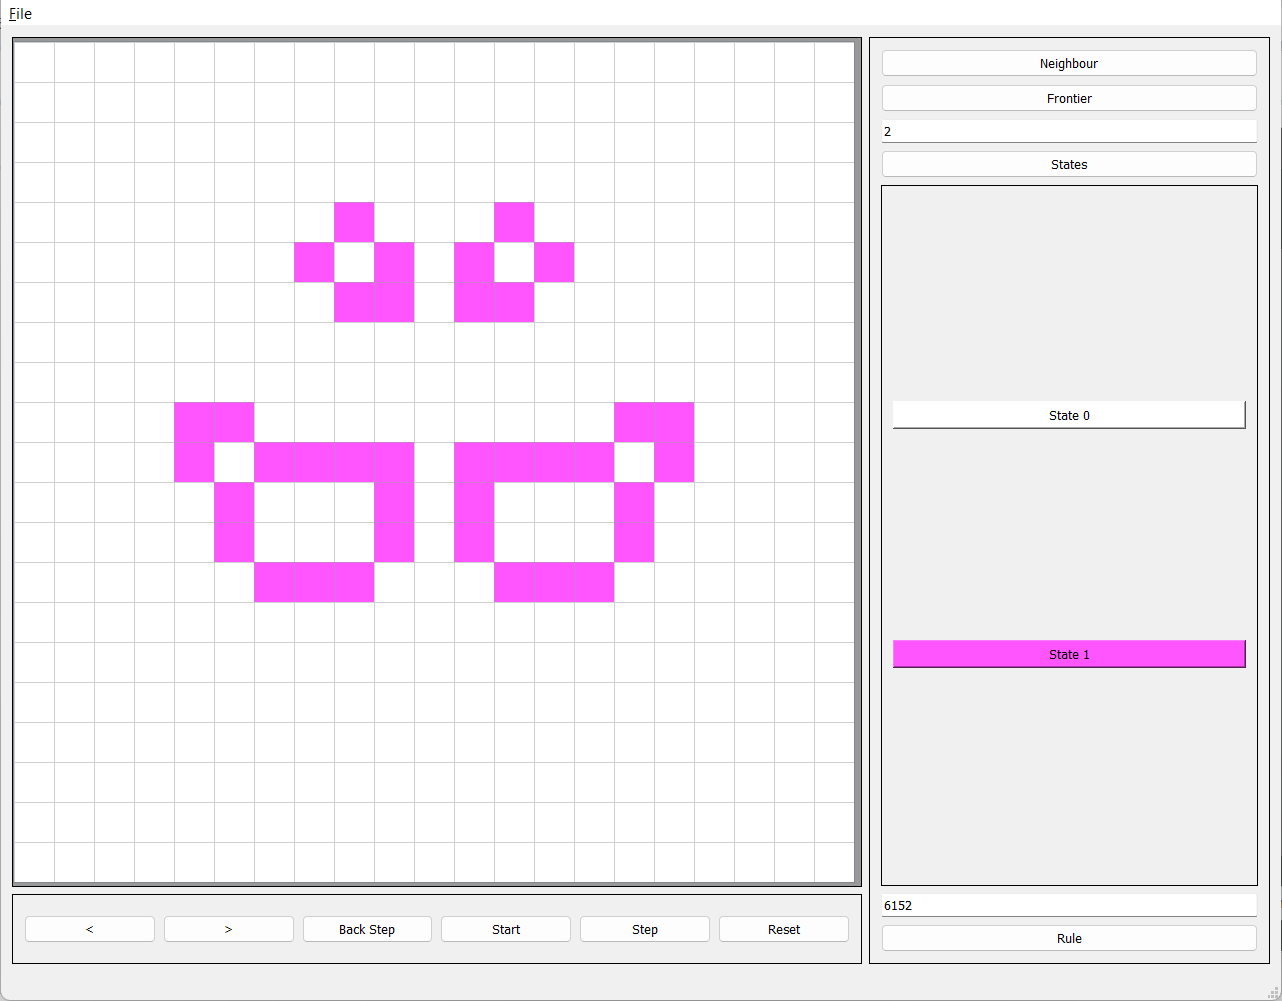
\includegraphics[width=0.9\linewidth]{img/ui_main.png}
		\caption{Interfaz de usuario principal.}
		\label{fig:ui_main}
	\end{figure}
	
	\item \textbf{Interfaz de vecindad}
	
	Esta interfaz permite al usuario definir la topología de la vecindad que determinará la dinámica del CA. Para ello, se presenta un espacio celular de menor tamaño en el cual se pueden activar o desactivar las celdas que formarán parte de la vecindad (Figura \ref{fig:ui_neighbour}).
	
	\begin{figure}[H]
		\centering
		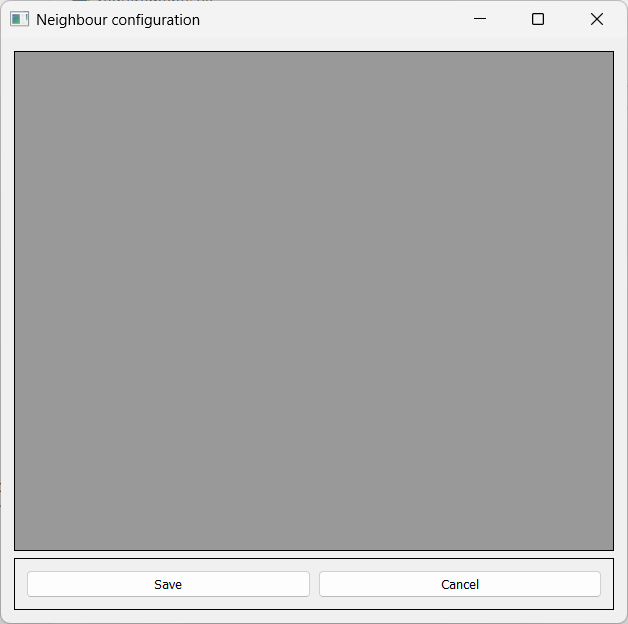
\includegraphics[width=0.65\linewidth]{img/ui_neighbour.png}
		\caption{Interfaz de usuario que define la vecindad.}
		\label{fig:ui_neighbour}
	\end{figure}
	
	\item \textbf{Interfaz para definir color}
	
	Esta ventana utiliza un componente nativo de \textbf{PyQt5} para la selección de colores. Permite al usuario asignar un color a cada estado del autómata (Figura \ref{fig:ui_color}).
	
	\begin{figure}[H]
		\centering
		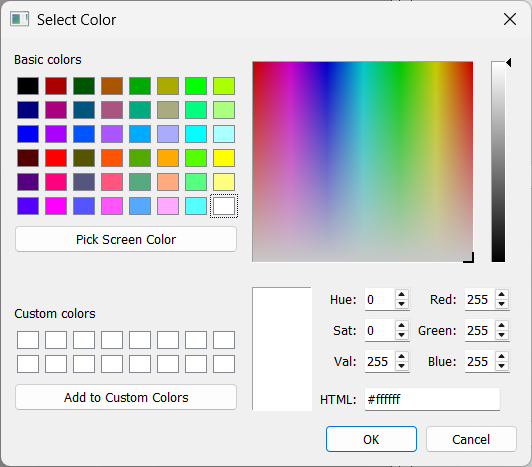
\includegraphics[width=0.4\linewidth]{img/ui_color.png}
		\caption{Interfaz de usuario para definir el color.}
		\label{fig:ui_color}
	\end{figure}
\end{itemize}
